
\chapter{JSON\label{appx:json}}

Acrônimo para JavaScript Object Notation (Notação de Objetos JavaScript), é um formato leve
para intercâmbio de dados computacionais, ou seja, é uma ponte entre a conversação entre
linguagens diferentes (\url{http://www.json.org/json-pt.html}).

\section*{Estrutura}

A representação de dados em JSON é bem simples. Temos essencialmente objetos, \textit{array}s,
par de chave e valor.

Um objeto é representado usando chaves da seguinte forma:

\begin{figure}[h]
\centering
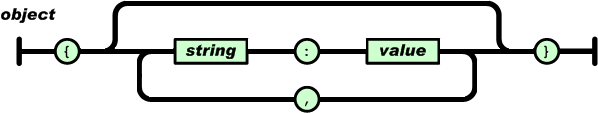
\includegraphics[scale=0.5]{img/json/object.png}
\caption{Objeto JSON}
\end{figure}

Já um \textit{array} é representado utilizando colchete:

\begin{figure}[h]
\centering
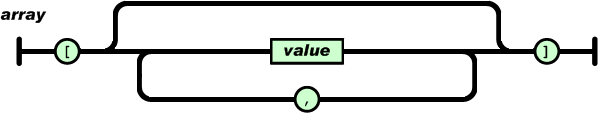
\includegraphics[scale=0.5]{img/json/array.png}
\caption{Array JSON}
\end{figure}

O valor (\textit{value}) pode ser uma \textit{string}, um número, ou \texttt{true} ou \texttt{false},
\texttt{null}, um \textit{array}, ou ainda um objeto. Estas estruturas podem estar aninhadas.

\begin{figure}
\centering
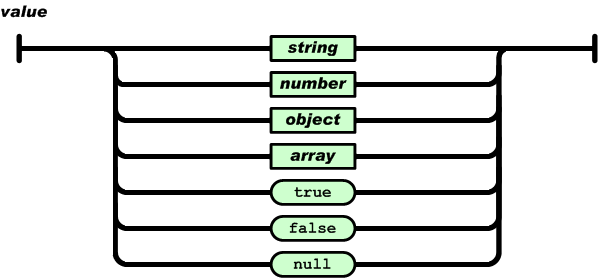
\includegraphics[scale=0.5]{img/json/value.png}
\caption{Possíveis valores}
\end{figure}

Uma \textit{string} é uma coleção de nenhum ou mais caracteres Unicode, envolvido entre aspas duplas usando
barras invertidas como caracter de escape. Um caracter está representando como um simples caracter
de \textit{string}. Uma cadeia de caracteres é parecida com uma cadeia de caracteres em C ou Java.

\begin{figure}
\centering
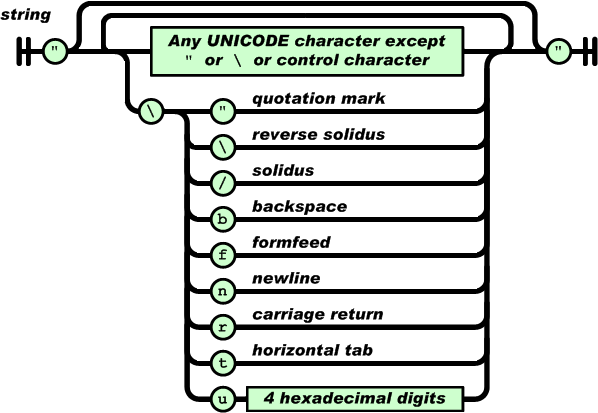
\includegraphics[scale=0.5]{img/json/string.png}
\caption{Formato de uma string}
\end{figure}

Um número é similar a um número em C ou Java, exceto quando não se usa os números octais ou hexadecimais.

\begin{figure}
\centering
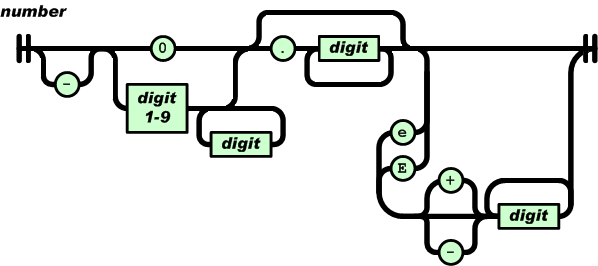
\includegraphics[scale=0.5]{img/json/number.png}
\caption{Formato de um número}
\end{figure}

\subsection*{Exemplo}

Para mostrar como funciona vamos a um exemplo bem prático. Utilizando um browser moderno, como o
chrome/chromium, abra o console que fica em \texttt{Ferramentas $\rightarrow$ Console JavaScript} ou
apenas \texttt{Ctrl + Shift + J}.

% TODO: mostrar exemplo criando um objeto, definindo atributos e imprimindo-os